\subsection{Metrics}
Although the field of heatmapping has received growing attention over the past decade, only little work has gone into the development of metrics. This is an issue, because absence of ground truth makes the search for metrics a non-trivial task --- while the lack of (reliable) metrics leads to flaws in the comparison of methods.

This subsection will provide a theoretical overview of commonly used metrics, \cref{metrics:aopc,metrics:faithfulness,metrics:roar}. Tools for verifying the reliability of metrics are given in~\fullref{metrics:sanity-checks}. A final overview and discussion are presented in~\fullref{metrics:discussion}

\subsubsection{Area Over the Perturbation Curve}\label{metrics:aopc} Proposed by~\fcite{WojciechSamek.2015}, \gls{aopc} is a generalization of the \textit{pixel flipping method} presented in~\cite[34\psqq]{Bach.2015}. \gls{aopc} measures the degradation of model-score for a certain input-sample, as input-variables are disabled in an iterative manner. Following either \gls{morf} or \gls{lerf} order. \gls{morf} and \gls{lerf} are extracted from the set of locations \[ \mathscr O = (\symbfit{r}_1, \symbfit{r}_2, \dots, \symbfit{r}_L), \] \todo{consider factoring this out as a general concept} which is ordered by decreasing relevance, i.e.\ informally: \[(i > j) \implies \text{relevance}(\symbfit{r}_i) < \text{relevance}(\symbfit{r}_j) \] Here, a location \( \symbfit{r}_p, p \in [1, L] \) must not be a single input, but could represent any constant multidimensional array of inputs (e.g.\ a \( 9\times9 \)-grid of pixels, as seen in the original paper).

\paragraph{Disabling Input Variables}
Disabling input variables comes with the risk of violating dataset statistics such as mean and variance. A sample-perturbation function that disables the region \(\symbfit{r}_k\) in the input-sample \(\symbfit{x}\) is formally introduced as \(g(\symbfit{x}, \symbfit{r}_k)\). \citeauthor{WojciechSamek.2015} propose to four sample-perturbation functions
\begin{itemize}
    \item replacing each value in \(\symbfit{r}_p\) by sampling a uniform distribution \(\mathscr U\)
    \item replacing each value in \(\symbfit{r}_p\) by sampling a Dirichlet distribution \(D\)
    \item replacing each value in \(\symbfit{r}_p\) by the average value of all samples for the current input-variable
    \item applying a Gaussian filter with \(\sigma = 3\) to \(\symbfit{r}_p\)
\end{itemize}
Note that the latter two, Gaussian filter and average value for the current input-variable, remove significantly less information from the input-sample than sampling from either \(\mathscr U\) or \(\mathscr D\).  Therefore (as removing information from the input-sample is the goal of disabling input variables) \citeauthor{WojciechSamek.2015} favor the first two, i.e.\ sampling \(\mathscr U\) or \(\mathscr D\).


\paragraph{Most Relevant and Least Relevant First}
\gls{morf} (\cref{eq:morf-base,eq:morf-recursive}) and \gls{lerf} (\cref{eq:lerf-base,eq:lerf-recursive}) are both defined recursively
\begin{align}
    \symbfit{x}^{(0)}_{\text{MoRF}} &= \symbfit{x}\label{eq:morf-base} \\
    \forall{1 \leq k \leq L}: \symbfit{x}^{(k)}_{\text{MoRF}} &= g(\symbfit{x}^{(k-1)}_{\text{MoRF}}, \symbfit{r}_k)\label{eq:morf-recursive} \\
    \symbfit{x}^{(0)}_{\text{LeRF}} &= \symbfit{x}\label{eq:lerf-base} \\
    \forall{1 \leq k \leq L}: \symbfit{x}^{(k)}_{\text{LeRF}} &= g(\symbfit{x}^{(k-1)}_{\text{LeRF}}, \symbfit{r}_{L+1-k})\label{eq:lerf-recursive}
\end{align}
where \(x^{(n)}_{\text{MoRF / LeRF}}, n \in [0, k]\) is the perturbed input-sample\todo{add \textit{input-sample} to glossary} at iteration \(n\) and by the respective order \gls{morf} / \gls{lerf}.

\paragraph{Area Over the Perturbation Curve}
The \gls{aopc} is then defined as
\[
    \text{AOPC}_M = \dfrac{\left< \sum_{k=0}^{L} f(\symbfit{x}^{(0)}_{M}) - f(\symbfit{x}^{(k)}_{M}) \right>}{L+1},
\]
where \(\left< \cdot \right>\) denotes the average over all input-samples\todo{define input-sample globally} in the \mbox{data set} and \(M \in \{\text{MoRF}, \text{LeRF}\}\). Informally, \gls{aopc} calculates the arithmetic mean of the average decrease in model-score\todo{define model-score globally. Model-score is more like model output, actually.} caused by disabling a range from \(0\) to \(L\) input variables\todo{define input variable globally}.

\subsubsection{Faithfulness}\label{metrics:faithfulness}
For faithfulness~\cite{AlvarezMelis.2018, Tomsett.2019}, as opposed to~\nameref{metrics:aopc}, model-outputs are computed with only a \textit{single} input-variable\todo{define input-variable globally} disabled at a time. Faithfulness is computed by taking Pearson correlation between the drop in model-output (when disabling the input-variable) and the relevance assigned to the input-variable by the heatmapping-method. Formally, given a sample \(\symbfit{x}\) with \(\left|\symbfit{x}\right|=n\) input-variables, an input-variable \(i\in \symbfit{x}\), the sample \(\symbfit{x}_i\) where \(i\) is disabled, a drop in model-output \(\Delta_i\) and a relevance for the input-variable \(R_i\):
\begin{align*}
    \Delta_i = f(\symbfit{x}) - f(\symbfit{x}_i)\\
    \text{Faithfulness}_{\symbfit{x}} = \frac{1}{n} \rho(R_i, \Delta_i)
\end{align*}
\todo{bring together \(\mathscr O and R_i\)}
gives the Faithfulness for a single image \(\symbfit{x}\). The Faithfulness over the full dataset is computed as
\[
    \text{Faithfulness} = \left<\rho(R, \Delta)\right>
\]
where, again, \(\left< \cdot \right>\) denotes the average over all input-samples in the \mbox{data set}


\subsubsection{Remove And Retrain}\label{metrics:roar}
\citeauthor{Hooker.2019} point out that previously mentioned metrics, \cref{metrics:aopc,metrics:faithfulness}, introduce new data distributions by artificially disabling input-variables. Therefore, violating one of the key assumptions in machine learning: `training and prediction data should arise from the same distribution'~\cite{McGaughey.2016}. Further, \citeauthor{Hooker.2019} show that model-performance degrades significantly slower when retraining in comparison to simply disabing input-variables, as can be seen in~\cref{fig:hooker-retraining-vs-no-retraining}.
\par
For each input-sample, a heatmap \(\mathscr H\) is produced. Where again,
\(\mathscr H\) is the set of feature importance estimates \( \{ e^{o}_{i} \}^N_{i=1} \)\todo{define this globally}. New training and test datasets are generated at different degradation levels \(t=\left[10, 30, 50, 70, 90 \right]\), with each \(t_i\) a percentage of input-variables per sample\todo{define the number of input-variables per sample globally}. To protect against random performance fluctuations, \citeauthor{Hooker.2019} retrain five models \(f_0^M(x_i), f_1^M(x_i),\ldots, f_4^M(x_i)\)\todo{Introduce notation for dataset and dataset degredation. Make clear that f(x) implies model \(f\) trained on x} for each metric \(M\) and each degradation method.

\paragraph{Keep And Retrain}
Similar to \gls{morf} and \gls{lerf}, \citeauthor{Hooker.2019} propose \gls{kar}. In \gls{kar}, input-variables are disabled in \gls{lerf} order.\todo{Maybe use lerf and morf globally, they are a good idea actually and also sound funny.}
\begin{figure*}[ht]
    \center{}
    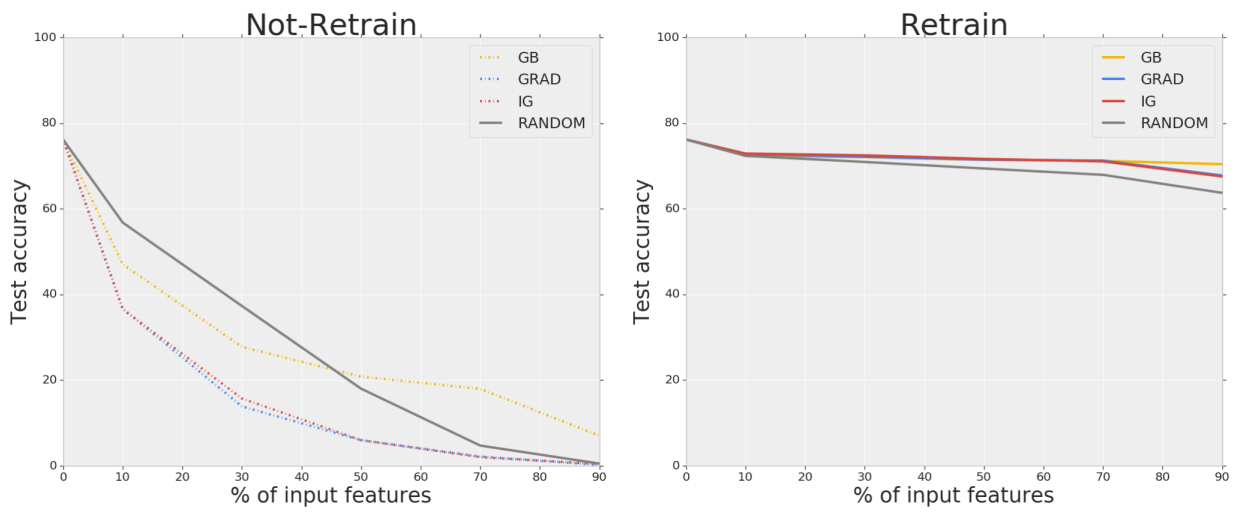
\includegraphics[width=\textwidth/2]{hooker-roar-retrain-nonretrain}
    \caption[The effect of retraining on model degredation in metrics.]{The figure shows the drastic decrease in model accuracy when disabling input-variables without retraining, but significantly smoothened when retraining is undertaken. Evaluated over Guided Backprop (GP), the unweighted gradient (GRAD), Integrated Gradients (IG) and random baseline.
    \textbf{Left:} evaluation of \gls{roar} without retraining. \textbf{Right:} evaluation of \gls{roar} with retraining. Adopted from~\cite{Hooker.2019}}\label{fig:hooker-retraining-vs-no-retraining}
\end{figure*}

%\subsubsection{Sensitivity-n}
%\citeauthor{Ancona.}\todo{There is Ancona and Acona. Merge them.}
%\blindtext[1]

\subsubsection{Sanity Checks for Metrics}\label{metrics:sanity-checks}
Just as for heatmaps, sanity checks were proposed for metrics~\cite{Tomsett.2019}. For determining whether a metric \textit{measures the intended property} and \textit{provides consistent results}, \citeauthor{Tomsett.2019} build upon three psychometric reliability tests (notice that both~\ref{itm:inter-rater} and~\ref{itm:inter-method} assume a \textit{fixed} metric)
\begin{description}
    \item[\namedlabel{itm:inter-rater}{Inter-rater reliability}{}] measures if heatmapping-methods are ranked consistently over the set of all input-samples.
    For calculation, \citeauthor{Tomsett.2019} refer to Krippendorff's \(\alpha\).
    \begin{description}
        \item[\(\alpha = 1\)] implies that a metric assigns the same ranking-order for the heatmapping-methods (i.e.\ if a heatmapping method is superior, it is consistently superior). 
        \item[\(\alpha = 0\)] implies that a metric assigns a random score for each heatmapping-method. Therefore, the fidelity of a heatmapping method cannot be predicted using the observed metric.
    \end{description} \todo{Read this again}
    \item[\namedlabel{itm:inter-method}{Inter-method reliability}{}] measures the correlation of metric-scores for different heatmapping methods over the set of all input-samples. For calculation, \citeauthor{Tomsett.2019} refer to Spearman's \(\rho\). A large \(\rho\) implies high inter-method reliability.
    \item[Internal consistency] measures if different metrics observe the same property (e.g.\ fidelity). For calculation, \citeauthor{Tomsett.2019} take the correlation (again, Spearman's \(\rho\)) of metric-scores from different metrics over the same heatmap.
\end{description}

\subsubsection{Discussion}\label{metrics:discussion}
Unfortunately, the discussed metrics either require significant computational effort (\gls{roar}, \cref{metrics:roar}) or have been shown unreliable (\gls{aopc} and Faithfulness, \cref{metrics:aopc,metrics:faithfulness})~\cite{Hooker.2019,Tomsett.2019}. Further, an evaluation of \gls{roar} in the like of \nameref{metrics:sanity-checks} has not been performed due to its computational complexity.
\par
This makes reliable comparison of methods almost impossible. For future research, evaluating the reliability of \gls{roar} and finding reliable, less computational complex metrics must be a priority. Proposing new methods is of subordinate importance, given that researchers remain unable to evaluate against preexisting approaches.